\documentclass[onecolumn,12pt]{asme2ej}
\usepackage{epsfig}\usepackage{amsmath}\usepackage{amsfonts}
\usepackage{amssymb}\usepackage{graphicx}\pagenumbering{arabic}
\usepackage{verbatim}\usepackage[utf8]{inputenc}\usepackage[portuguese]{babel}
\providecommand{\keywords}[1]{\small\textbf{\textit{Keywords---}} #1}
\usepackage{comment}
\usepackage[backend=biber,style=numeric,sorting=none]{biblatex}
\usepackage{fancyhdr}\usepackage{pifont}
\usepackage{tikzsymbols}\usepackage{placeins}
\usepackage{rotating}\usepackage{longtable}
\setcounter{tocdepth}{4}\setcounter{secnumdepth}{4}
\pagestyle{fancy}\fancyhf{}\rfoot{Página \thepage}
\addbibresource{mybib.bib} 

\title{Processo Decisório Multicritério para a Avaliação de Projetos de Tecnologia da Informação\\Projeto Diskify\\Análise de Viabilidade}

\author{Gustavo Hammerschmidt\affiliation{PUCPR - Ciência da Computação\\g.hammerschmidt@pucpr.edu.br}}

\begin{document}

\maketitle $\\$

\FloatBarrier
\begin{figure}[h]
    \centering
    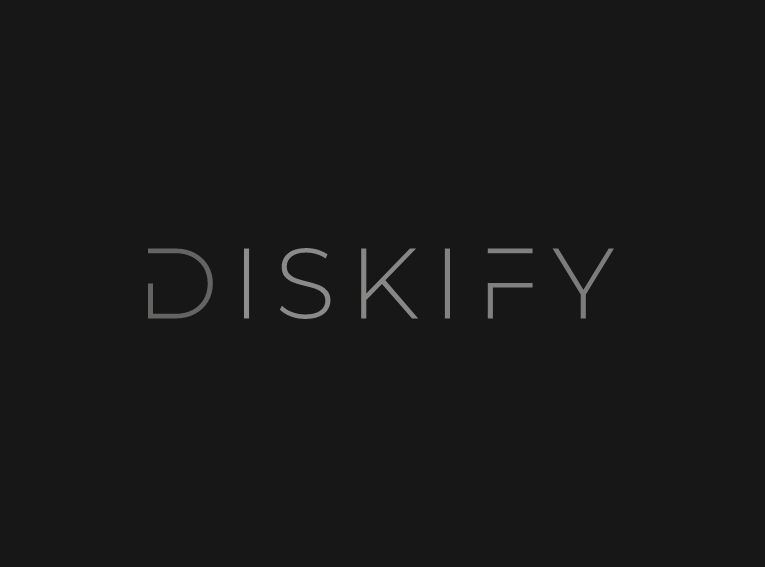
\includegraphics[width=13cm]{ks/diskify.PNG}
    \label{fig:head}
\end{figure}
\FloatBarrier \newpage

$\\ \\ \\ \\ \\ \\$ $\\ \\ \\ \\ \\ \\$ $\\ \\ \\ \\ \\ \\$
\begin{abstract}{\it 
Tokens não-fungíveis (NFTs) se tornaram um atrativo para muitos mercados, um notável caso de sucesso de tecnologia baseada  em blockchain. NFTs são baseadas em contratos inteligentes (Smart Contracts) e são usadas para a definição e transferência de direitos de propriedade, representando vários tipos de dados. O projeto Diskify aproxima a indústria da música de seus fãs, promovendo escassez de conteúdo e eliminando intermediários como aplicativos de streaming e produtoras.
}\end{abstract} \newpage \tableofcontents \newpage

\section{Introdução}

Desde 8 de março de 2020, o mercado de criptomoedas tem crescido e atingido máximas históricas mensalmente (COINMARKETCAP, 2021). A procura por esses tipos de ativos aumentou devido à preocupação de investidores com o futuro da economia em meio à corrente situação pandêmica. Os motivos que os levam a optar por essas moedas são, geralmente, desconfiança do lastro de suas moedas fiat – isso deve-se à quebra do acordo de Bretton Woods em 15 de agosto de 1971: quando o governo do presidente americano, Richard Nixon, encerrou a convertibilidade do dólar em ouro; até antes dessa mudança, um cidadão americano poderia ir ao banco e trocar cada dólar que tivesse por uma quantia em gramas de ouro fixa. Perceba que, a partir deste momento, o dólar se torna uma moeda fiduciária (moeda fiat), uma moeda sem lastro em algum metal precioso, como ouro ou prata, mas com lastro na confiança de seus usuários em quem as emite, bancos centrais em serviço do Estado. Países como Japão, Suíça e Rússia compraram ouro dos Estados Unidos pós o rompimento do sistema de Bretton Woods para ficaram independentes de crises americanas e possuírem reservas de valor próprias. Os eventos ocorridos em 2020 com relação à COVID-19 não possuem precedentes históricos, estamos mais conectados e sintonizados nas notícias sobre o que está acontecendo ao redor do mundo. Como muitas empresas foram fechadas temporariamente e outras para sempre, pessoas ficaram sem empregos e precisavam de subsídios para se manter durante esse período, de janeiro a junho do mesmo ano, mais de 20\% de todo o dinheiro existente em 2019 foi impresso (ROBERTSON, 2020), isso implica em todas as reservas físicas até então se desvalorizando o equivalente em porcentagem; pois imprimir dinheiro não é gerar valor, e inflacionar não equivale em estimular o consumo. Fatos como este impulsionam investidores mais conservadores a buscarem alternativas fora de seu perfil de risco para proteger seu capital, a busca por moedas deflacionárias como o Bitcoin – uma moeda deflacionária é um ativo que tende a se manter em quantidade limitada e escassa, ou seja, a oferta da moeda é fixa e a demanda por ela tende a aumentar com o tempo; no caso do bitcoin, por ser a primeira delas, muitos mineradores armazenaram suas chaves privadas em discos rígidos ou em carteiras aos quais perderam o acesso, portanto, na prática, ainda que o número máximo de bitcoins seja 21 milhões de moedas, há um número menor delas em circulação – o que corrobora com o aspecto deflacionário e a propulsiona em termos de valor de mercado; muitos críticos afirmam que o bitcoin, em especial, é uma pirâmide financeira e que precisa de lastro do Estado para funcionar, porém, não percebem que o lastro do bitcoin remanesce na matemática pois o abastecimento da moeda é fixo e ela mantém os registros das trocas entre usuários na blockchain, evitando que transações falsas sejam realizadas. Afinal, o objetivo de uma moeda é facilitar trocas e manter suas reservas de valor.

\FloatBarrier
\begin{figure}[h]
    \centering
    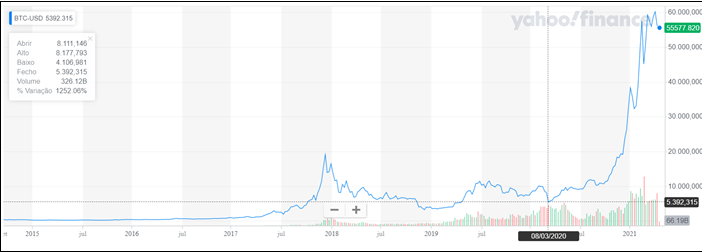
\includegraphics[width=15cm]{fs/f11.PNG}
    \caption{Valorização do Bitcoin entre 04/03/2020 e 20/04/2021.}
    \label{fig:f11}
\end{figure}
\FloatBarrier

Considerando as criptomoedas (descentralizadas) como o futuro da economia, aplicações de finanças decentralizadas (DeFi – decentralized finance) e NFTs (NAPOLETANO, 2021) obtiveram um enfoque da comunidade de investidores cripto, tendo aumentado o seu valor de mercado durante a pandemia também. Elas visam a remover um intermediário de produtos financeiros, tornando o indivíduo em seu próprio banco ou corretora. NFTs, tokens não fungíveis, são colecionáveis com direito de propriedade: o uso deles tem sido adotado por fãs da arte moderna, sendo muitas obras digitais salvas em rede blockchain e suas NFTs negociadas entre usuários. O artista conhecido como Beeple leiloou uma de suas artes digitais por 69 milhões de dólares na casa de leilão Christie’s em 11 de março de 2021 (Figura 1-2), ele está entre os três artistas vivos mais valiosos atualmente. Uma pergunta recorrente é por que alguém compraria uma imagem que pode ser facilmente replicada ou por que alguém pagaria para ter algo que pode ver gratuitamente; a resposta para esse tipo de comportamento é que as pessoas são coletoras, gostam de colecionar objetos mais pelo valor que veem neles do que uma finalidade ou utilidade tão somente, pois o valor de objetos é sempre subjetivo e está fora dele à mercê das trocas voluntárias entre indivíduos; igualando-se aos motivos pelos quais um comprador pagaria preços exorbitantes na Monalisa, mesmo que esta obra seja amplamente conhecida e já replicada, pois cabe aqui a ideia de propriedade sobre o objeto. Com as várias aplicabilidades de um NFT, alguns projetos almejam integrá-las em contratos de propriedade física, como uma rede de NFTs para apartamentos que permita uma troca fácil e direta, outros desafiando os padrões da arte contemporânea.

\FloatBarrier
\begin{figure}[h]
    \centering
    
\includegraphics[width=12cm]{fs/f12.PNG}
    \caption{NFT de Beeple negociada na Christie’s: Everydays – The First 5000 Days.}
    \label{fig:f12}
\end{figure}
\FloatBarrier

Diskify é um projeto que integra a indústria musical à tecnologia das NFTs. Músicos menos populares ficam sujeitos a gravadoras e aos direitos autorais que elas têm sobre suas produções. Com a plataforma proposta, os artistas podem vender álbuns – havendo um limite de cópias definido pelo artista, o que aumenta a raridade do produto –, eliminando a porcentagem da receita líquida que vai para as gravadoras e gerando uma fonte de renda alternativa para que não dependam de seus shows apenas. Como há uma raridade em cada álbum, fãs podem acordar um preço pelo produto de forma subjetiva – pois a plataforma Diskify em muito se assemelha à uma Exchange de valores ou um Marketplace digital – e, se a posteriori decidirem revendê-los, haverá um mecanismo conhecido como royalties utilizado em NFTs de arte digitais: é uma forma de recompensar o artista pelo seu trabalho, a cada troca feita uma porcentagem do preço acordado é repassada ao músico. 

Portanto, o projeto Diskify é uma plataforma de livre acesso e negociação de bens digitais que possibilita trocas de álbuns musicais por criptomoedas, integrando o direito de propriedade sobre o álbum em NFTs e as armazenando em carteiras digitais cripto, se o usuário assim desejar. Com uma NFT, o fã pode baixar para seu dispositivo as músicas e reproduzi-las, mas, caso queira revender seu token, as terá removidas de seu dispositivo. Isso não impede que algum usuário regrave as músicas e as poste em alguma outra plataforma, mas isso configura pirataria e continuará sendo um item de menor valor subjetivo do que o original.

\FloatBarrier
\begin{figure}[h]
    \centering
    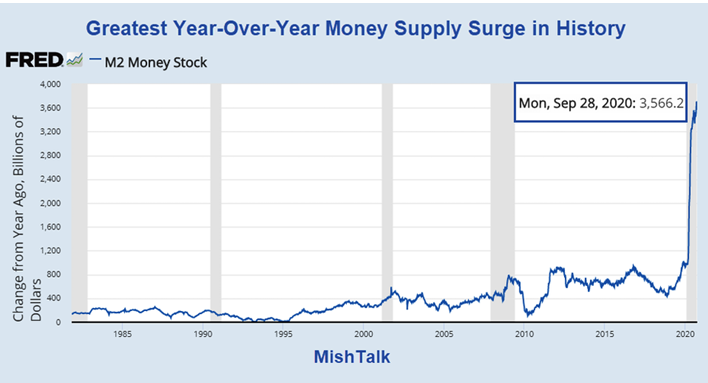
\includegraphics[width=12cm]{fs/f13.PNG}
    \caption{2020, o ano de maior impressão de dólares na história.}
    \label{fig:f13}
\end{figure}
\FloatBarrier

\subsection{Modelo do Plano de Negócios e Personas}

O modelo se segue abaixo:

\FloatBarrier
\begin{figure}[h]
    \centering
    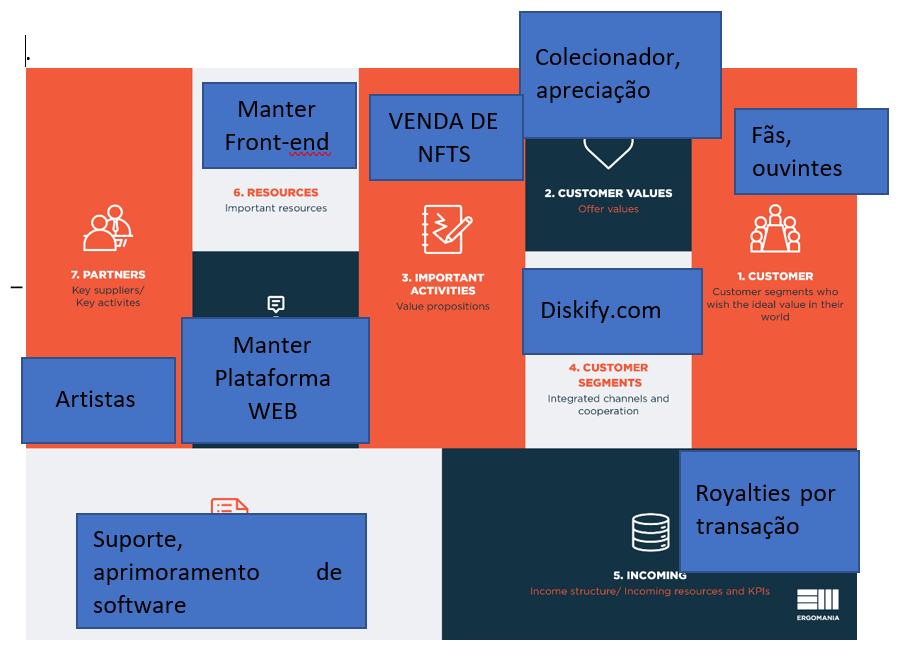
\includegraphics[width=12cm]{fs/BMC.PNG}
    \caption{Business Model Canvas.}
    \label{fig:bmc}
\end{figure}
\FloatBarrier

Como a empresa pretende mitigar custos e gerar inovação:

\FloatBarrier
\begin{figure}[h]
    \centering
    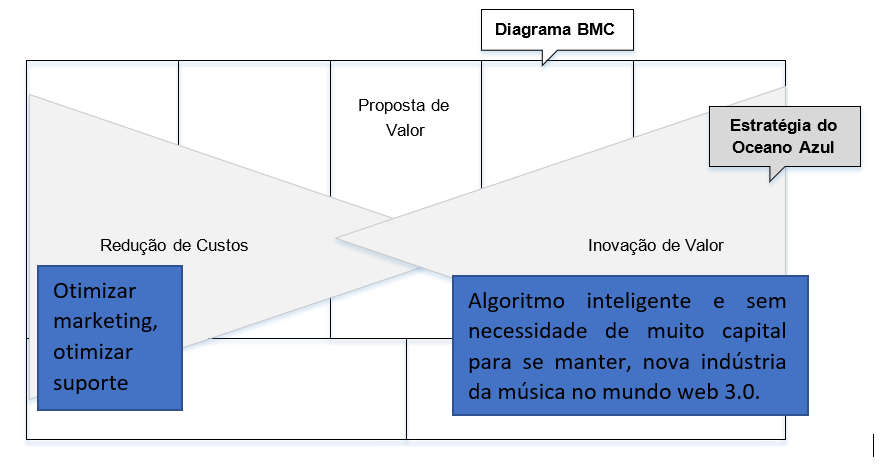
\includegraphics[width=12cm]{fs/bmc2.PNG}
    \caption{Soluções: mitigação de custo.}
    \label{fig:bmc2}
\end{figure}
\FloatBarrier

Questões-chave sobre o nosso modelo:

\FloatBarrier
\begin{figure}[h]
    \centering
    
\includegraphics[width=12cm]{fs/g1.PNG}
    \caption{Questões-chave: parte 1.}
    \label{fig:qc1}
\end{figure}
\FloatBarrier

\FloatBarrier
\begin{figure}[h]
    \centering
    
\includegraphics[width=12cm]{fs/g2.PNG}
    \caption{Questões-chave: parte 2.}
    \label{fig:qc2}
\end{figure}
\FloatBarrier

\FloatBarrier
\begin{figure}[h]
    \centering
    
\includegraphics[width=12cm]{fs/g3.PNG}
    \caption{Questões-chave: parte 3.}
    \label{fig:qc3}
\end{figure}
\FloatBarrier

Matriz de Inovação de Valor:

\FloatBarrier
\begin{figure}[h]
    \centering
    
\includegraphics[width=12cm]{fs/h1.PNG}
    \caption{Matriz de inovação de valor.}
    \label{fig:h1}
\end{figure}
\FloatBarrier

Personas:

\FloatBarrier
\begin{figure}[h]
    \centering
    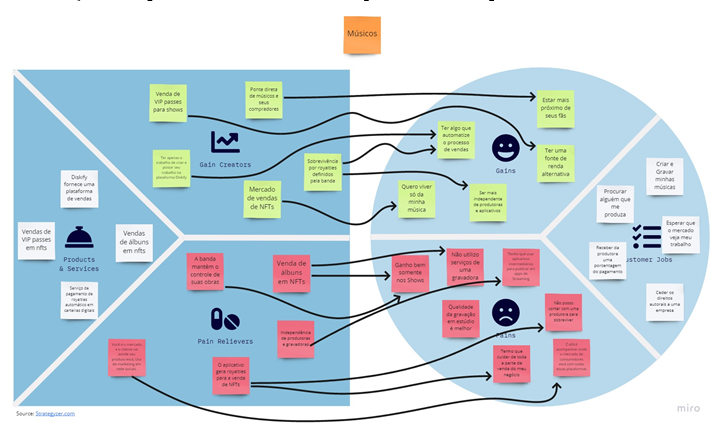
\includegraphics[width=12cm]{fs/pers1.PNG}
    \caption{Modelo para o Canvas da Proposta de Valor para Músicos. Fonte: Strategyzer.}
    \label{fig:p1}
\end{figure}
\FloatBarrier

\FloatBarrier
\begin{figure}[h]
    \centering
    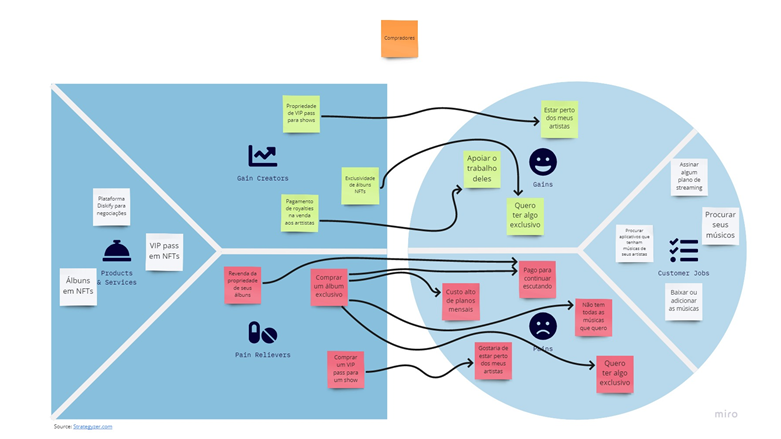
\includegraphics[width=12cm]{fs/pers2.PNG}
    \caption{Modelo para o Canvas da Proposta de Valor para Consumidores. Fonte: Strategyzer.}
    \label{fig:p2}
\end{figure}
\FloatBarrier

\section{Empresa e Problema de Decisão}

A {\it Diskify} é um marketplace descentralizado de NFTs de áudio. Nesta seção, descreveremos o processo de escolha de projeto para adesão ao modelo de negócio da empresa: o nosso próximo produto a ser comercializado pelos usuários na rede.
 
\subsection{Descrição da Empresa}

A razão de ser da {\it Diskify} tem como objetivo a criação de um Marketplace de negociação de NFTs de álbuns musicais, a facilitação para músicos de venderem suas obras de forma independente de produtoras e a criação de uma fonte alternativa de renda.  

O público-alvo do projeto Diskify se divide em duas personas: Músico e Comprador. Músico é todo aquele indivíduo que se interessa por publicar seus trabalhos artísticos e musicais na plataforma de forma a automatizar o processo de vendas e pagamento de royalties. Comprador é todo fã interessado em consumir algum álbum produzido por artistas. As entrevistas feitas limitaram-se aos dois perfis e às suas dores. Nossas personas e seu comportamento no canvas de proposta de valor foram figurados na seção 1.1.

A descrição de negócio da Diskify é um projeto que integra a indústria musical à tecnologia das NFTs. Músicos menos populares ficam sujeitos a gravadoras e aos direitos autorais que elas têm sobre suas produções. Com a plataforma proposta, os artistas podem vender álbuns – havendo um limite de cópias definido pelo artista, o que aumenta a raridade do produto –, eliminando a porcentagem da receita líquida que vai para as gravadoras e gerando uma fonte de renda alternativa para que não dependam de seus shows apenas. Como há uma raridade em cada álbum, fãs podem acordar um preço pelo produto de forma subjetiva – pois a plataforma Diskify em muito se assemelha à uma Exchange de valores ou um Marketplace digital – e, se a posteriori decidirem revendê-los, haverá um mecanismo conhecido como royalties utilizado em NFTs de arte digitais: é uma forma de recompensar o artista pelo seu trabalho, a cada troca feita uma porcentagem do preço acordado é repassada ao músico. Portanto, o projeto Diskify é uma plataforma de livre acesso e negociação de bens digitais que possibilita trocas de álbuns musicais por criptomoedas, integrando o direito de propriedade sobre o álbum em NFTs e as armazenando em carteiras digitais cripto, se o usuário assim desejar. Com uma NFT, o fã pode baixar para seu dispositivo as músicas e reproduzi-las, mas, caso queira revender seu token, as terá removidas de seu dispositivo. Isso não impede que algum usuário regrave as músicas e as poste em alguma outra plataforma, mas isso configura pirataria e continuará sendo um item de menor valor subjetivo do que o original. 

Um ponto desprezado por produtores e gravadoras: a independência e vontade dos músicos em se autoproduzir e gerar renda, sem abusos de receita ou cláusulas de contrato leoninas; e, também, a desassociação da ideia de que uma empresa detém os direitos de propriedade intelectual sobre sua arte: também, dessa forma, aproximando o consumidor de seus artistas com a possibilidade de deter a propriedade de conteúdos exclusivos. As entrevistas levantaram pontos esperados e ajudaram a estipular que pessoas interessadas em apoiar algum artista também estão dispostas a comprar colecionáveis. Durante as entrevistas, um novo canal de renda para a plataforma Diskify veio à tona, segundo à perspectiva da equipe, seria interessante adicionar a ideia de passes VIP para shows como NFTs para venda na plataforma. Os passes seriam emitidos pelos artistas, tendo a distinção de passes vitalícios que permitiriam aos seus donos de participaram de backstages (espaço ao lado ou atrás do palco em que fãs ou ajudantes ficam durante os shows), e, se não conseguissem participar de algum evento, poderia alugar ou revender o seu passe – sempre, nessas negociações, realizando royalties para os artistas e uma porcentagem ao projeto Diskify. O entrevistado 7 disse não gostar de ter que fazer todo o processo de venda de seus álbuns e arrecadação, abordando a exata intenção do projeto; enquanto isso, o entrevistado 1 disse que gostaria de ter uma fonte de renda com NFTs. Ter a visão dos músicos entrevistados ajudou a adicionar termos e compreender dinâmicas de mercado e subsistência pelas as quais eles se conformam, e como criar um modelo de negócio disruptivo – a Diskify. O projeto Diskify evita ser um impasse na comunicação entre as personas citadas, isso significa que nossa prioridade se dá na garantia da propriedade intelectual das obras. Uma vez que o álbum esteja disponível à venda, a empresa só terá acesso à NFT dele para fins de checagem ao direito de propriedade intelectual.

As condições de desempenho consideradas essenciais para o projeto são, já que o propósito da empresa é remover os {\it middlemen} (intermediários) que existem entre músicos e seus fãs no que tange a distribuição de suas músicas e propriedade intelectual das obras, adotamos, como filosofia da empresa, a ética libertária de conduta dos indivíduos e a sua auto-soberania como prioridades no desenvolvimento do projeto. Afinal, a empresa precisa ser um marketplace auto-sustentável e descentralizado. Logo, a empresa focará em sempre se manter como contra-parte das relações músicos-fãs e evitará intervir nelas, somente quando houver o descumprimento das políticas de termos de serviços da nossa empresa.

\subsection{Descrição do Problema de Decisão}

Temos que decidir qual será o nosso projeto dentro da plataforma para atrair mais usuários e aumentar a utilidade dos nossos produtos como um todo, afinal, queremos possibilitar o uso normal do aplicativo como se fosse da Web 2.0 com os pontos positivos da Web 3.0 e possibilitar novas funcionalidades - possíveis somente na Web 3.0. Para isso, teremos que decidir sobre os projetos: 1) Projeto Podcast, inserção de podcasts ao mundo NFT dentro da nossa plataforma; 2) Projeto Community, aumento dos recursos da nossa comunidade, estruturação do nosso lado de suporte ao cliente com o uso da comunidade; 3) Projeto Youtube Song Property Share, possibilitar que suas músicas possam ser usadas nas suas produções audiovisuais, como vídeos no youtube, sem implicação de direitos autorais, fazendo com que os artistas tenham reconhecimento; e 4) Projeto Platform Sponsored Artists, selecionar artistas para patrocinarmos e aumentarmos os royalties produzidos por nós. Com isso, pretendemos aumentar a nossa lucratividade com base nos critérios selecionados abaixo.

\subsection{Critérios de Decisão}

São os nossos critérios de decisão, os seguintes: 1) Mercadológico, 2) Técnico e 3) Financeiro. Os subcritérios de 1 são: macroambiente, forças de porter e demanda; os de 2, HW - tecnologia, SW - tecnologia e pessoal; os de 3, ROIA, TIR e PayBack.

\subsection{Alternativas de Decisão}

As alternativas de decisão citadas são: Projeto Podcast (1), Projeto Community (2), Projeto Youtube Song Property Share (3) e Projeto Platform Sponsored Artists (4). Para facilitar o entendimento das tabelas, vamos nos referir a eles com relação aos seus números.

\section{Tomada de Decisão com Multicritérios}

Nesta seção, descreveremos o nosso processo AHP, a árvore do processo e o algoritmo para ele.

\subsection{Considerações Gerais}

Apresentaremos a árvore AHP e as avaliações pareadas para essas subseções; considere os números de cada projeto como dito na seção anterior para facilitar a visibilidade das tabelas. As consolidações e visão geral dos resultados obtidos do algoritmo definido para o AHP serão mostradas na análise de resultados.

\subsection{Analytic Hierarchy Process (AHP)}

A seguir, a árvore AHP do nosso processo decisório.

\FloatBarrier
\begin{sidewaysfigure}[h]
    \centering
    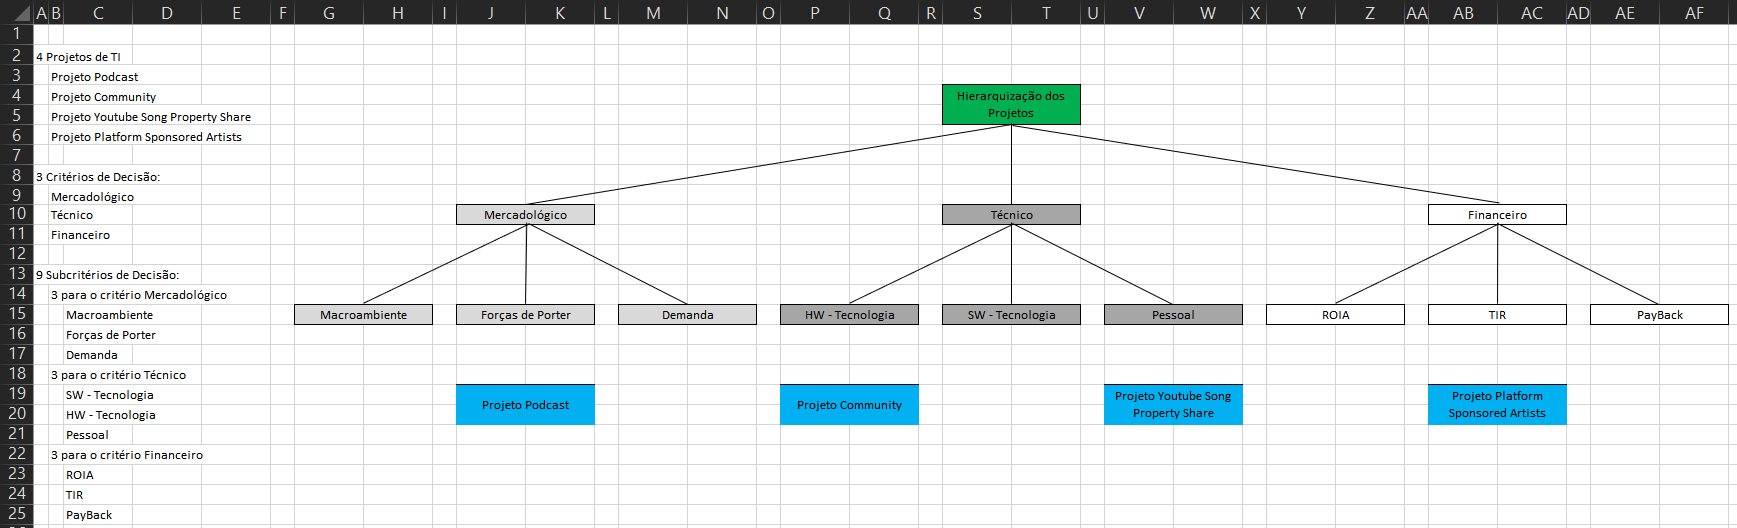
\includegraphics[width=24cm]{zs/AHPTree.PNG}
    \caption{Árvore AHP.}
    \label{fig:ahptree}
\end{sidewaysfigure}
\FloatBarrier \newpage

\subsection{Algoritmo para o AHP}

Nosso algoritmo consiste de matrizes de preferência para cada critério, com comparações pareadas, a comparação das alternativas é realizada utilizando uma escala própria, que varia de 1 a 9. A seguir, as avaliações pareadas para o processo.

\FloatBarrier
\begin{figure}[h]
    \centering
    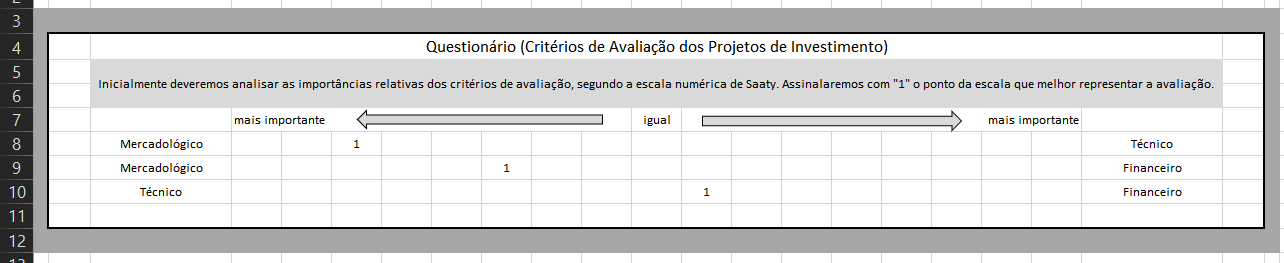
\includegraphics[width=18cm]{zs/AP1.PNG}
    \caption{Avaliação Pareada: Critérios.}
    \label{fig:ap1}
\end{figure}
\FloatBarrier 

\FloatBarrier
\begin{figure}[h]
    \centering
    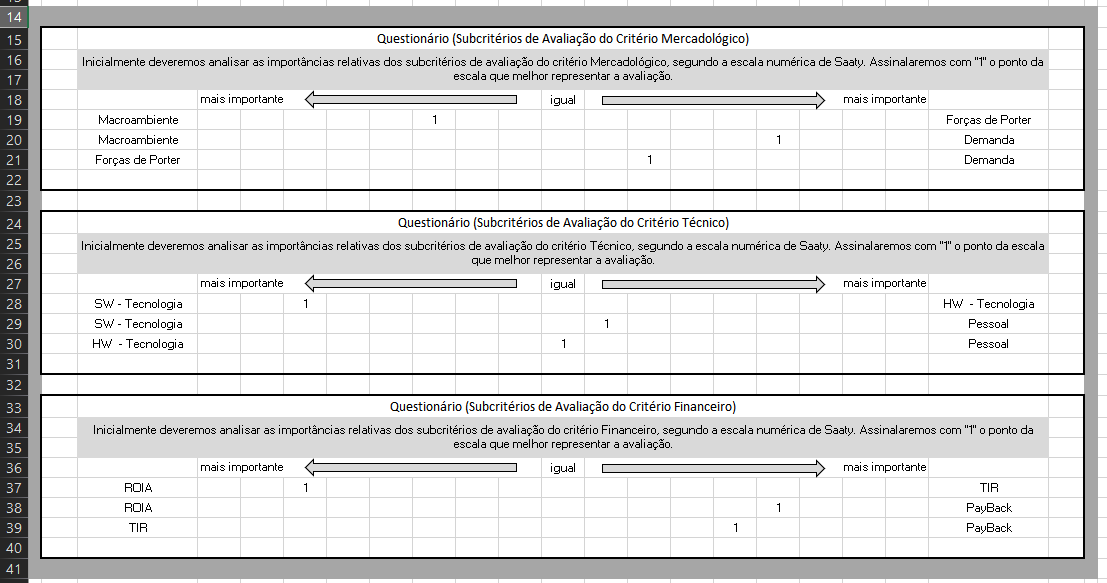
\includegraphics[width=18cm]{zs/AP2.PNG}
    \caption{Avaliação Pareada: Subcritérios.}
    \label{fig:ap2}
\end{figure}
\FloatBarrier 

\FloatBarrier
\begin{figure}[h]
    \centering
    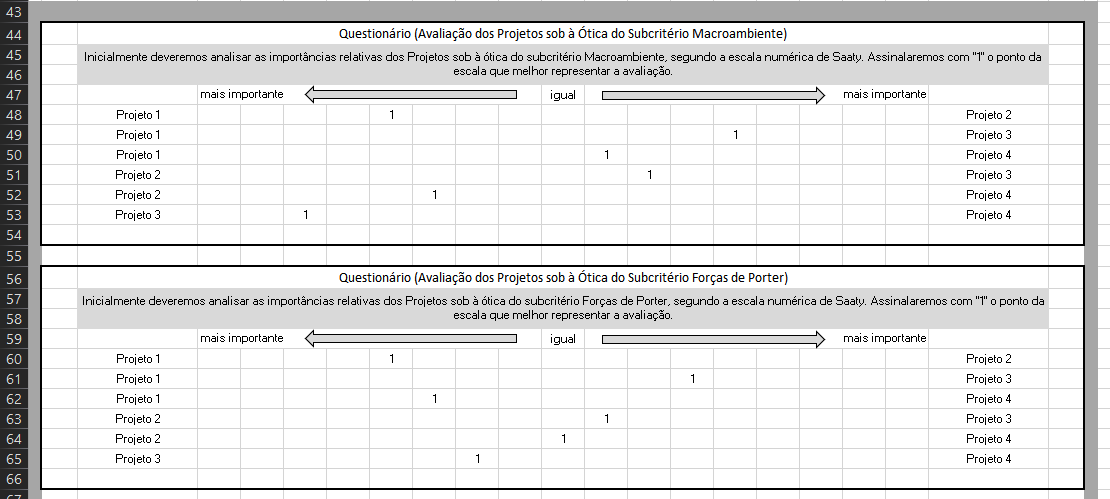
\includegraphics[width=18cm]{zs/AP3a.PNG}
    \caption{Avaliação Pareada: Projetos vs. Subcritérios Mercadológicos.}
    \label{fig:ap3a}
\end{figure}
\FloatBarrier 

\FloatBarrier
\begin{figure}[h]
    \centering
    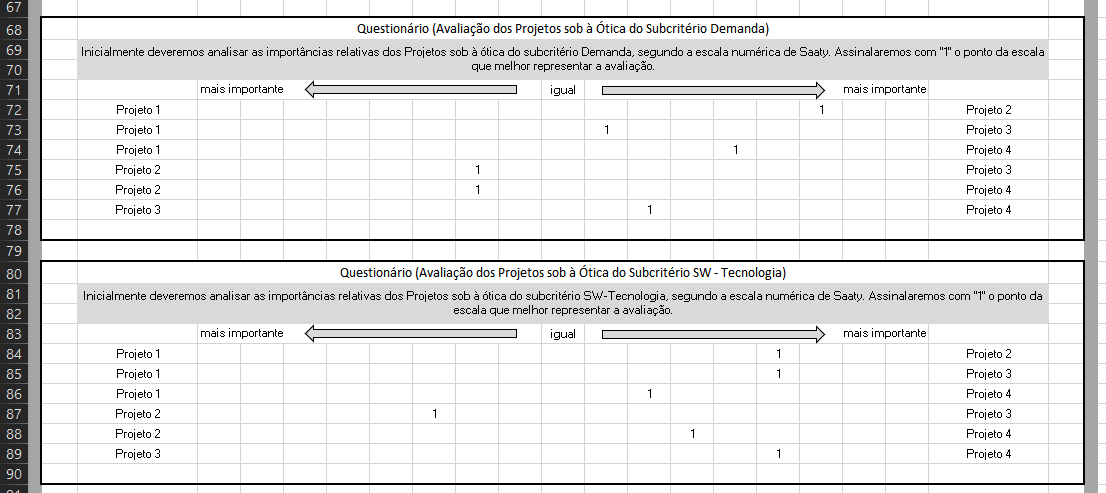
\includegraphics[width=18cm]{zs/AP3b.PNG}
    \caption{Avaliação Pareada: Projetos vs Subcritérios Mercadológicos e Técnicos.}
    \label{fig:ap3b}
\end{figure}
\FloatBarrier 

\FloatBarrier
\begin{figure}[h]
    \centering
    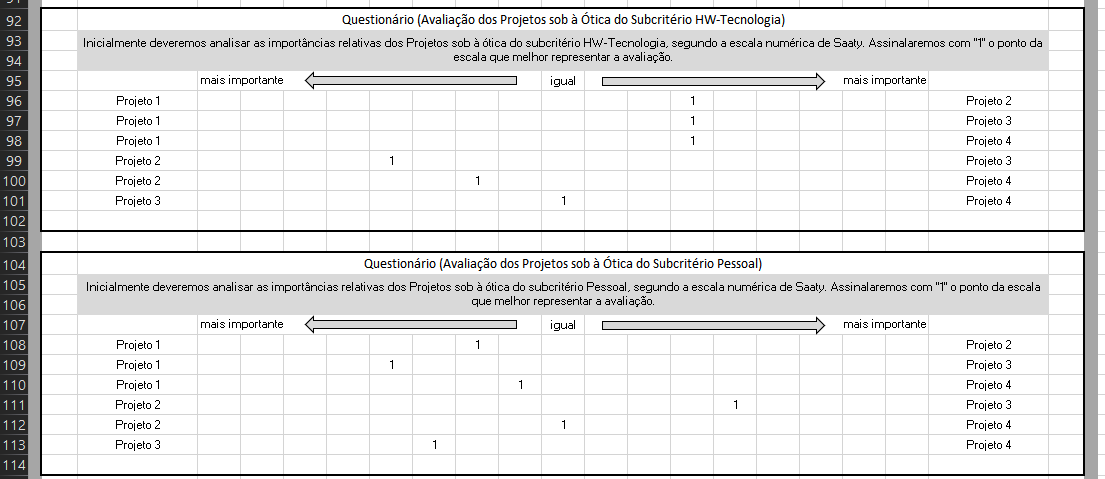
\includegraphics[width=18cm]{zs/AP3c.PNG}
    \caption{Avaliação Pareada: Projetos vs Subcritérios Técnicos.}
    \label{fig:ap3c}
\end{figure}
\FloatBarrier 

\FloatBarrier
\begin{figure}[h]
    \centering
    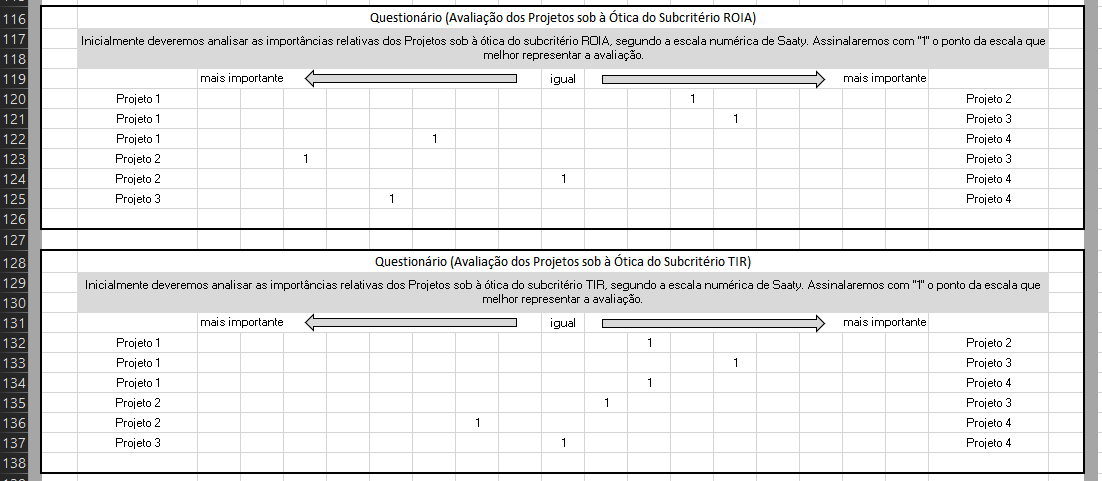
\includegraphics[width=18cm]{zs/AP3d.PNG}
    \caption{Avaliação Pareada: Projetos vs Subcritérios Financeiros.}
    \label{fig:ap3d}
\end{figure}
\FloatBarrier 

\FloatBarrier
\begin{figure}[h]
    \centering
    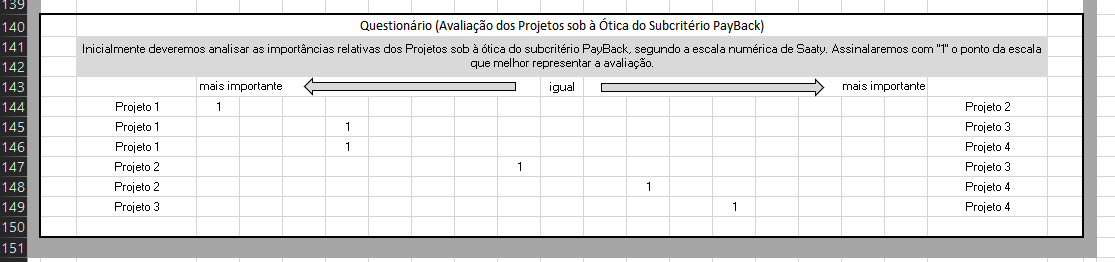
\includegraphics[width=18cm]{zs/AP3e.PNG}
    \caption{Avaliação Pareada: Projetos vs Subcritérios Financeiros.}
    \label{fig:ap3e}
\end{figure}
\FloatBarrier 

\section{Modelo Multicritério de Decisão}

Nesta seção, mostraremos os resultados obtidos com base na categorização de prioridades definidas nas avaliações acima.

\subsection{AHP para Hierarquização das Alternativas de Decisão}

Os resultados obtidos para os critérios, subcritérios e alternativas de decisão, com base nas estimativas feitas nas avaliações, são mostrados a seguir, segundo o processo AHP.

\subsubsection{1º Nível: Critérios de Decisão}

\FloatBarrier
\begin{figure}[h]
    \centering
    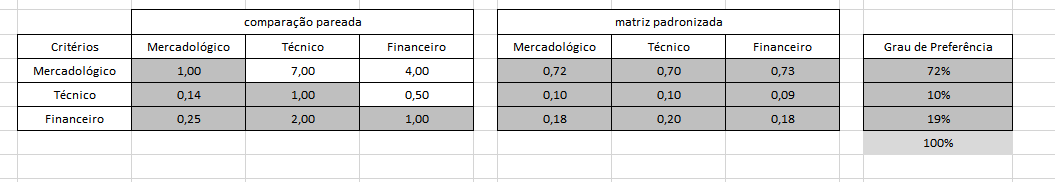
\includegraphics[width=18cm]{zs/Criterios.PNG}
    \caption{Comparação pareada dos critérios com base nas avaliações.}
    \label{fig:criterios}
\end{figure}
\FloatBarrier 

\subsubsection{2º Nível: Subcritérios de Decisão de Cada Critério}

\FloatBarrier
\begin{figure}[h]
    \centering
    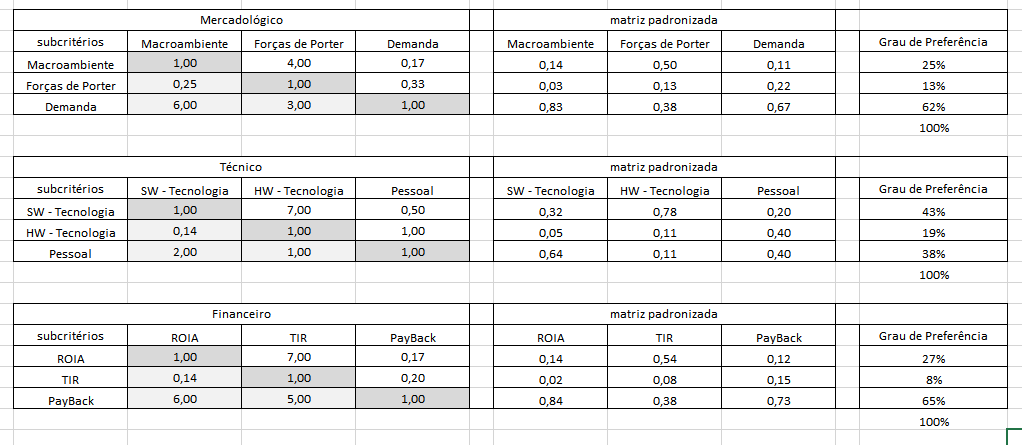
\includegraphics[width=18cm]{zs/Subcriterios.PNG}
    \caption{Comparação pareada dos subcritérios com base nas avaliações.}
    \label{fig:subcriterios}
\end{figure}
\FloatBarrier 

\subsubsection{3º Nível: Alternativas de Decisão x Subcritérios de Decisão}

\FloatBarrier
\begin{figure}[h]
    \centering
    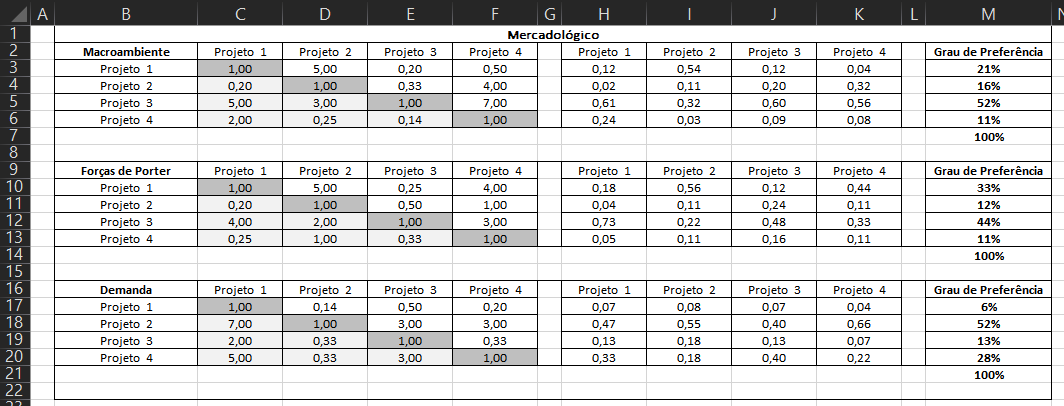
\includegraphics[width=18cm]{zs/projmercadologico.PNG}
    \caption{Comparação pareada dos projetos: subcritério mercadológico.}
    \label{fig:pmercadologico}
\end{figure}
\FloatBarrier 

\FloatBarrier
\begin{figure}[h]
    \centering
    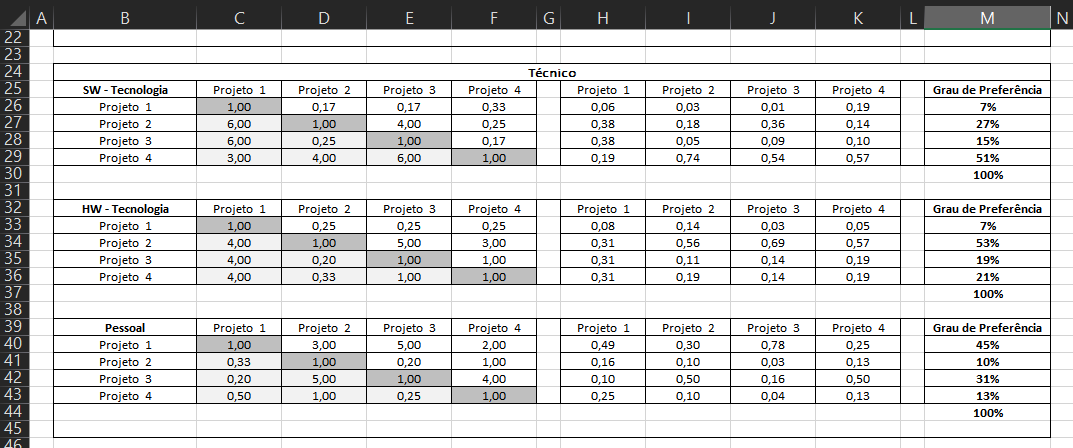
\includegraphics[width=18cm]{zs/projtecnico.PNG}
    \caption{Comparação pareada dos projetos: subcritério técnico.}
    \label{fig:ptecnico}
\end{figure}
\FloatBarrier 

\FloatBarrier
\begin{figure}[h]
    \centering
    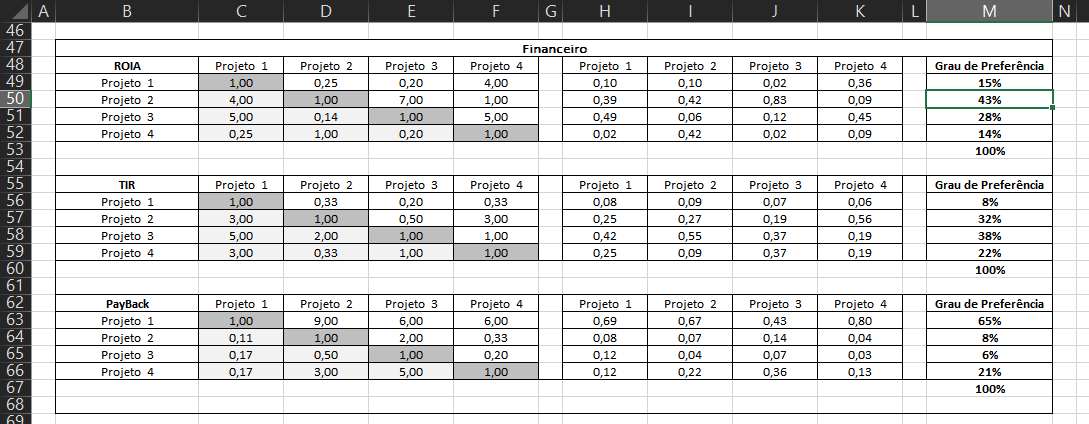
\includegraphics[width=18cm]{zs/projfinanceiro.PNG}
    \caption{Comparação pareada dos projetos: subcritério financeiro.}
    \label{fig:pfinanceiro}
\end{figure}
\FloatBarrier 

\subsection{Análise dos Resultados}

A seguir, a consolidação 1:

\FloatBarrier
\begin{figure}[h]
    \centering
    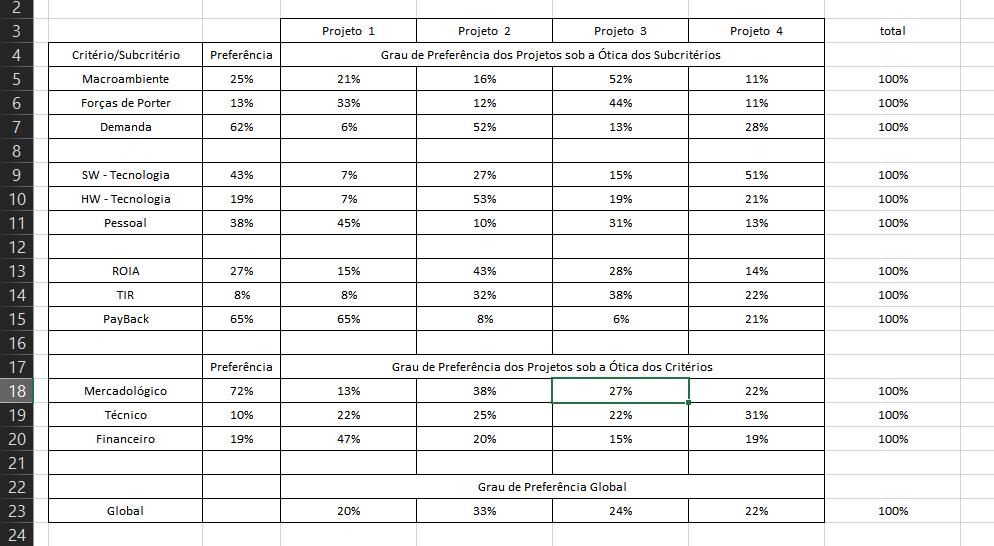
\includegraphics[width=16cm]{zs/Consolidacao1.PNG}
    \caption{Consolidação 1.}
    \label{fig:consolidacao1}
\end{figure}
\FloatBarrier 

A seguir, a consolidação 2:

\FloatBarrier
\begin{figure}[h]
    \centering
    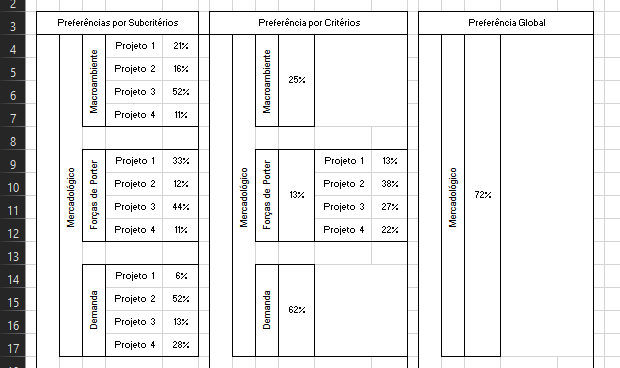
\includegraphics[width=16cm]{zs/Consolidacao2a.PNG}
    \caption{Consolidação 2a.}
    \label{fig:consolidacao2a}
\end{figure}
\FloatBarrier 

\FloatBarrier
\begin{figure}[h]
    \centering
    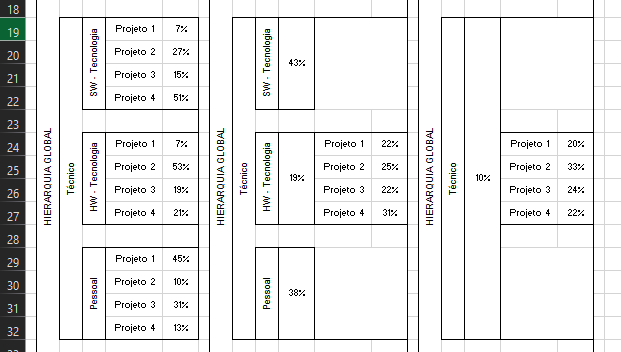
\includegraphics[width=16cm]{zs/Consolidacao2b.PNG}
    \caption{Consolidação 2b.}
    \label{fig:consolidacao2b}
\end{figure}
\FloatBarrier 

\FloatBarrier
\begin{figure}[h]
    \centering
    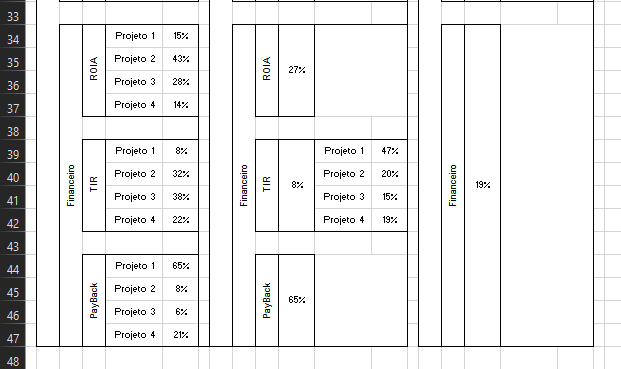
\includegraphics[width=16cm]{zs/Consolidacao2c.PNG}
    \caption{Consolidação 2c.}
    \label{fig:consolidacao2c}
\end{figure}
\FloatBarrier 

A seguir, as visões gerais mercadológica, técnica e financeira:

\FloatBarrier
\begin{figure}[h]
    \centering
    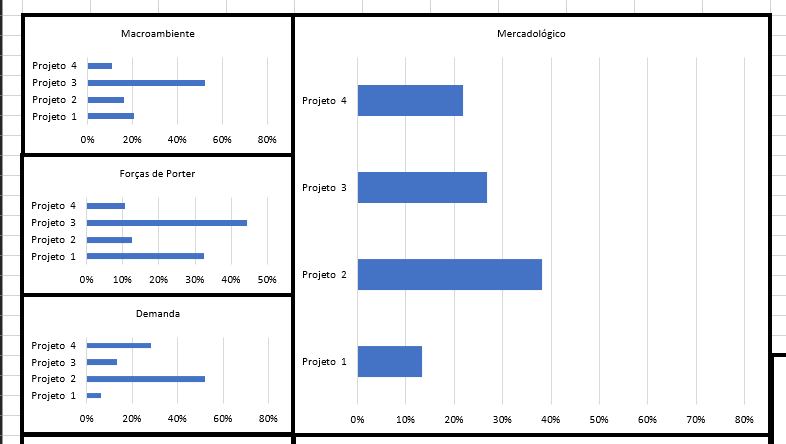
\includegraphics[width=12cm]{zs/vg_mercadologico.PNG}
    \caption{Visão Geral Mercadológica.}
    \label{fig:vgm}
\end{figure}
\FloatBarrier 

\FloatBarrier
\begin{figure}[h]
    \centering
    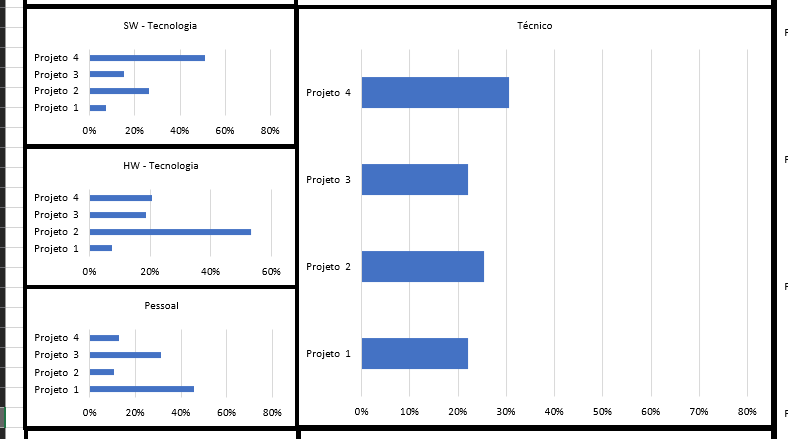
\includegraphics[width=12cm]{zs/vg_tecnico.PNG}
    \caption{Visão Geral Técnica.}
    \label{fig:vgt}
\end{figure}
\FloatBarrier 

\FloatBarrier
\begin{figure}[h]
    \centering
    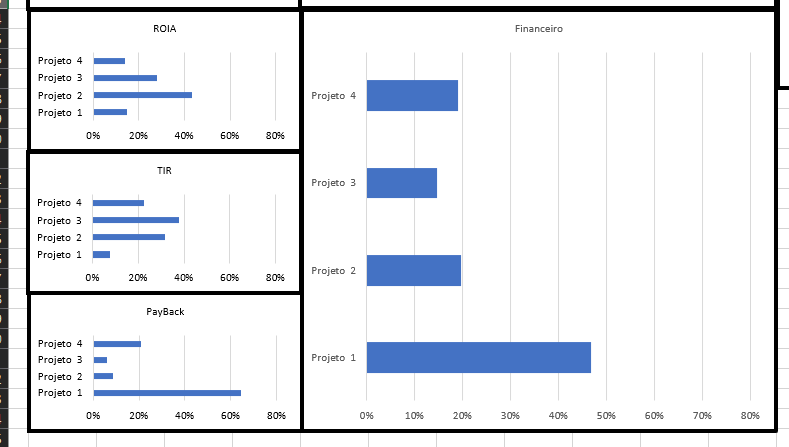
\includegraphics[width=12cm]{zs/vg_financeiro.PNG}
    \caption{Visão Geral Financeira.}
    \label{fig:vgf}
\end{figure}
\FloatBarrier 

A seguir, a visão geral global: 

\FloatBarrier
\begin{figure}[h]
    \centering
    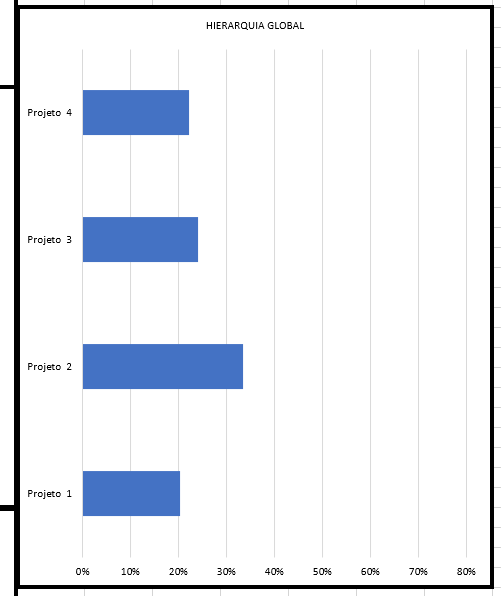
\includegraphics[width=10cm]{zs/vg_global.PNG}
    \caption{Visão Geral Global.}
    \label{fig:vgg}
\end{figure}
\FloatBarrier 

Pode-se analisar que PayBack, demanda e software foram os subcritérios mais preferíveis de cada critério, e que houve um equilíbrio de afinidade de cada projeto para cada subcritério - difícil de ver um destaque grande entre os projetos. No entanto, o projeto 2 teve um melhor proveito dos subcritérios e obteve destaque global maior aos demais, sendo que o projeto 1 teve destaque no critério financeiro, o projeto 3 no critério mercadológico (depois do projeto 2) e o projeto 4 no critério técnico.

\section{Conclusão}

Como visto nos resultados obtidos, o projeto 2 (Projeto Community) é o que teve maior relevância global dentre os projetos avaliados no processo AHP, a empresa deve focar seus esforços primariamente em desenvolver uma comunidade atrativa e intuitiva para a plataforma como forma de suporte e conhecimento dos usuários. A empresa também deve executar em segundo plano o projeto 1 (Projeto Podcast) como forma de trabalhar o lado financeiro da empresa, e focar nele quando tiver concluído o projeto 2. Caso haja necessidade e tempo, devemos priorizar o projeto 3 em vez do projeto 4 porque ele cobre a área mercadológica da empresa com mais ênfase, logo é ótimo para estimular o consumo dos nossos produtos e nos afastar dos concorrentes. O projeto 4 deve ser ignorado momentaneamente até uma eventual necessidade de aplicar novos projetos à plataforma.

\section{Adicionais}

Alguns adicionais sobre o projeto e informações relevantes para o entendimento da filosofia da DAO e suas motivações enquanto comunidade.

\subsection{Elicitando as referências}

Conhecimentos sobre o mercado financeiro sobre preços dos cripto-ativos e sobre fatos históricos relacionados podem ser encontrados em: \cite{rrf1}\cite{rrf12}\cite{rrf8}\cite{rrf11}\cite{rrf4}. Conhecimentos sobre a tecnologia por trás das NFTs: \cite{rrf5}
\cite{rrf9}\cite{rrf7}. Conhecimentos sobre o mundo DeFi: \cite{rrf3}\cite{rrf6}. Curiosidades sobre o artista Beeple e sua obra mais valiosa: \cite{rrf2}.

\subsection{Link para Vídeo sobre a Implementação do Projeto}

Este link é para o vídeo da implementação das fundações da aplicação desenvolvida e sua lógica de funcionamento, explicando cada item do código e sua relevância na automatização dos contratos: https://youtu.be/UnzlorkFw9g.

\newpage
\printbibliography  

\end{document}
